\documentclass[11pt]{article}

\usepackage[a4paper,margin=1in]{geometry}
\usepackage{amsmath,amssymb,amsfonts}
\usepackage{booktabs}
\usepackage{graphicx}
\usepackage{multirow}
\usepackage{array}
\usepackage{siunitx}
\usepackage{xcolor}
\usepackage{hyperref}
\usepackage{enumitem}
\usepackage{caption}
\usepackage{subcaption}
\usepackage{algorithm}
\usepackage{algorithmic}
\usepackage{longtable}

\hypersetup{
  colorlinks=true,
  linkcolor=black,
  citecolor=black,
  urlcolor=black
}

\sisetup{
  round-mode=places,
  round-precision=4,
  detect-weight=true,
  detect-family=true
}

\title{Urban Traffic Forecasting and Congestion Analysis with Paper-Inspired Spatio-Temporal Graph Models and a Traceable Analysis Agent}
\author{Project Manuscript for Reproducible Portfolio Evaluation}
\date{}

\begin{document}
\maketitle

\begin{abstract}
Short-term traffic forecasting is a fundamental task in intelligent transportation systems because accurate speed prediction supports congestion monitoring, operational diagnosis, and offline decision support. This paper presents a reproducible urban traffic forecasting and congestion analysis system built around four components: time-series preprocessing, spatio-temporal graph forecasting, congestion-oriented error diagnosis, and a traceable analysis agent. The system evaluates naive baselines, temporal-only recurrent models, educational graph models, and paper-inspired full spatio-temporal graph models on the METR-LA traffic sensor dataset. Unlike demonstration-only traffic chatbots, the proposed project emphasizes strict temporal splitting, physical road-topology alignment, multi-horizon and multi-seed evaluation, graph-structure ablation, congestion subset analysis, and structured reporting. Experimental results show that the paper-inspired GraphWaveNetFull model achieves the lowest mean absolute error across 15-, 30-, and 60-minute horizons, reducing MAE relative to the LastValue baseline by 0.5539, 0.6438, and 0.8986, respectively. Graph-structure ablation further indicates that graph information is generally beneficial over identity graphs, although the relative advantage of physical, correlation, and adaptive graphs depends on the model and horizon. The analysis remains deliberately conservative: the implemented models are paper-inspired engineering realizations rather than official reproductions, and the results are not claimed to be state-of-the-art. The system is intended for reproducible learning, internship portfolio demonstration, and offline traffic analytics rather than real-time traffic control.
\end{abstract}

\textbf{Keywords:} traffic forecasting; spatio-temporal graph neural networks; Graph WaveNet; STGCN; METR-LA; congestion analysis; reproducible machine learning; analysis agent

\section{Introduction}
Urban road networks exhibit strong temporal inertia, recurrent daily patterns, and spatial dependencies caused by road connectivity and congestion propagation. Short-term traffic forecasting therefore requires models that can simultaneously handle temporal dynamics and graph-structured interactions among sensors. In practical machine learning projects, however, it is easy to overstate model performance by comparing only against weak baselines, using random time splits that leak future information, reporting a single aggregate metric, or presenting synthetic demonstrations as if they were real-world experiments. This work addresses these issues by building a reproducible forecasting and analysis pipeline that treats baselines, graph structure, failure cases, and reporting as first-class components.

The project is named \emph{Urban Traffic Forecasting \& Congestion Analysis Agent}. Its objective is not to reproduce official benchmark leaderboards or claim industrial deployment readiness. Instead, it aims to demonstrate a rigorous engineering workflow for intelligent transportation: preparing real traffic sensor data, aligning physical topology with sensor order, training multiple forecasting models, evaluating across horizons and seeds, diagnosing congestion-related failure modes, and exposing results through a dashboard and a traceable analysis agent. This framing is important because a useful portfolio project should show not only that a model can run, but also that its results can be trusted, inspected, and communicated honestly.

The main contributions are summarized as follows:
\begin{itemize}[leftmargin=*]
  \item A reproducible real-data pipeline for METR-LA style traffic sensor data, including HDF5 loading, DCRNN-style adjacency loading, node alignment, and explicit reporting of dropped or reordered nodes.
  \item A structured model hierarchy covering naive baselines, temporal-only models, educational graph models, and paper-inspired full spatio-temporal graph models.
  \item Implementations of GraphWaveNetFull and STGCNFull that retain core architectural ideas such as dilated causal convolution, gated temporal convolution, graph message passing, residual/skip connections, and adaptive adjacency where appropriate.
  \item A multi-horizon, multi-seed experiment protocol with MAE, RMSE, raw MAPE, and masked MAPE, where conclusions prioritize MAE, RMSE, and masked MAPE due to the instability of raw MAPE near zero speeds.
  \item Graph-structure ablation and congestion subset evaluation to determine whether graph models improve not only overall averages but also low-speed, speed-drop, high-variance, and normal-flow regimes.
  \item A traceable analysis layer that can answer model-comparison and diagnostic questions from stored artifacts without fabricating unavailable results.
\end{itemize}

\section{Problem Formulation}
A road sensor network is represented as a graph $G=(V,E,A)$, where $V$ is the set of $N$ traffic sensors, $E$ is the set of road-topology relations, and $A\in\mathbb{R}^{N\times N}$ is the adjacency matrix. At time step $t$, the traffic state is denoted by $X_t\in\mathbb{R}^{N\times F}$, where $F$ is the number of features. In the METR-LA experiments reported here, the primary observed feature is speed.

Given an input window of length $T$,
\begin{equation}
  X_{t-T+1:t}=\{X_{t-T+1},\ldots,X_t\}\in\mathbb{R}^{T\times N\times F},
\end{equation}
the forecasting task is to predict future speeds over a horizon $H$:
\begin{equation}
  \hat{Y}_{t+1:t+H}=f_\theta(X_{t-T+1:t}, A)\in\mathbb{R}^{H\times N}.
\end{equation}
The experiments use $T=12$, corresponding to one hour of historical observations under a five-minute sampling interval, and $H\in\{3,6,12\}$, corresponding to 15-, 30-, and 60-minute prediction horizons.

Time-series data must be split chronologically rather than randomly. Random splitting would allow future temporal patterns to influence training and validation, creating an unrealistic estimate of forecasting performance. Therefore, the project uses a 70\%/10\%/20\% chronological train/validation/test split. Missing values are imputed using forward fill, backward fill, and training-set statistics, while normalization parameters are fitted only on the training segment.

\section{System Overview}
The system consists of five interacting layers.

\subsection{Data Layer}
The data layer supports both synthetic demonstration data and real METR-LA/PEMS-BAY style data. Synthetic data is used only for quick-start, CI, and smoke testing. Real experiments rely on externally prepared traffic files and adjacency matrices. For METR-LA, the traffic file is read from HDF5 and the physical topology is read from a DCRNN-style \texttt{adj\_mx.pkl} file. If the traffic DataFrame column order differs from the adjacency sensor order, the data tensor is reordered according to the adjacency sensor IDs. If one source contains sensors missing from the other, the intersection is used and a node alignment report is saved. This is essential because graph neural networks assume that the $i$-th node in the data tensor corresponds exactly to the $i$-th row and column in the adjacency matrix.

\subsection{Forecasting Layer}
The forecasting layer compares four groups of models: naive baselines, temporal-only neural networks, educational graph models, and paper-inspired full graph models. The hierarchy is intentionally explicit so that complex models are judged against strong simple alternatives.

\subsection{Analysis Layer}
The analysis layer computes standard forecasting metrics, graph-ablation summaries, congestion subset metrics, and failure diagnostics. It avoids using raw MAPE as the primary conclusion metric because traffic speeds can approach zero, causing percentage errors to explode. Masked MAPE and absolute-error metrics are therefore emphasized.

\subsection{Agent Layer}
The agent layer is a rule-based, traceable analysis assistant. It selects registered read-only tools to answer questions such as whether full models outperform LastValue, whether graph structure is useful, why raw MAPE is high, and which model performs best on congestion subsets. The agent is not a traffic-control system and does not issue signal-control actions.

\subsection{Visualization Layer}
The dashboard and exported figures provide compact views of model performance, horizon effects, graph ablation, parameter-efficiency tradeoffs, and congestion subset behavior. The figures used in this manuscript are generated from stored experiment artifacts rather than manually entered values.

\section{Models}
\subsection{Naive and Statistical Baselines}
\textbf{LastValue} predicts each future speed as the last observed speed in the input window. It is a strong short-term baseline because traffic speed often has high temporal inertia. A deep model that fails to outperform LastValue should not be described as effective for short-horizon forecasting.

\textbf{HistoricalAverage} predicts future speeds using the average speed in the input history window. \textbf{SeasonalNaive} is designed to exploit time-of-day recurrence when sufficient historical seasonal context is available; otherwise, it falls back to HistoricalAverage. In the present experiments, HistoricalAverage and SeasonalNaive have identical aggregate results, indicating that the available implementation context did not provide additional seasonal advantage beyond the historical average fallback.

\subsection{Temporal-Only Neural Models}
\textbf{LSTM} and \textbf{GRU} flatten node-feature states into temporal vectors and model the sequence using recurrent networks. These models capture temporal dependencies but do not explicitly use road topology. They serve as controls for determining whether graph-based spatial modeling provides additional value.

\subsection{Educational Graph Models}
\textbf{STGCNImproved} and \textbf{GraphWaveNetLite} are simplified graph models. They are useful for explaining temporal/spatial decomposition and for debugging the pipeline, but they are not intended to faithfully reproduce the original papers.

\subsection{Paper-Inspired GraphWaveNetFull}
GraphWaveNetFull implements the main design ideas of Graph WaveNet: start convolution, dilated causal temporal convolution, gated activation, diffusion graph convolution over multiple supports, residual and skip connections, end convolution, and adaptive adjacency. For an input hidden state $Z$, a gated temporal unit computes
\begin{equation}
  Z' = \tanh(\Theta_f * Z) \odot \sigma(\Theta_g * Z),
\end{equation}
where $*$ denotes temporal convolution and $\odot$ denotes element-wise multiplication. Graph diffusion uses powers of normalized supports, including identity, normalized adjacency, transposed adjacency, and optionally an adaptive adjacency:
\begin{equation}
  A_{adaptive}=\operatorname{softmax}(\operatorname{ReLU}(E_1E_2)),
\end{equation}
where $E_1$ and $E_2$ are learnable node embeddings. This implementation is paper-inspired and educational; it is not an official reproduction of the original Graph WaveNet training protocol.

\subsection{Paper-Inspired STGCNFull}
STGCNFull follows the ST-Conv block idea: temporal gated convolution, graph convolution, another temporal gated convolution, residual connection, layer normalization, and dropout. The graph convolution uses Chebyshev-style $K$-order message passing, where node states are aggregated from progressively wider neighborhoods. This model is also paper-inspired rather than an official reproduction.

\section{Experimental Protocol}
\subsection{Dataset}
The experiments use METR-LA, a traffic speed dataset with 207 sensors. The processed tensor has shape $[T,N,F]$ with $N=207$ and $F=1$ for speed. The physical road-topology adjacency is loaded from the DCRNN-style adjacency file and aligned to the HDF5 sensor column order. Synthetic runs are excluded from the main conclusions.

\subsection{Training Configuration}
All neural models are trained with chronological train/validation/test splits. The RTX 5090 configuration uses batch size 64, up to 100 epochs, Adam-style optimization through the PyTorch training loop, weight decay $10^{-4}$, gradient clipping with norm 5.0, mixed precision when CUDA is available, and early stopping with patience 20. The primary training loss is masked MAE. Each model is evaluated over horizons $H\in\{3,6,12\}$ and seeds $\{42,43,44\}$.

\subsection{Metrics}
The main metrics are MAE, RMSE, and masked MAPE:
\begin{align}
  \operatorname{MAE} &= \frac{1}{M}\sum_i |y_i-\hat{y}_i|,\\
  \operatorname{RMSE} &= \sqrt{\frac{1}{M}\sum_i (y_i-\hat{y}_i)^2},\\
  \operatorname{masked\ MAPE} &= \frac{100}{|\Omega|}\sum_{i\in\Omega}\left|\frac{y_i-\hat{y}_i}{y_i}\right|.
\end{align}
The set $\Omega$ excludes invalid or near-zero denominators according to the masking rule. Raw MAPE is stored for transparency but is not used as the primary conclusion metric because traffic speeds near zero can produce unstable percentage errors.

\section{Main Results}
Table~\ref{tab:main_results} reports multi-seed aggregate results on METR-LA. GraphWaveNetFull achieves the best MAE at all horizons, followed by STGCNFull and GraphWaveNetLite. LastValue remains a strong baseline but is no longer the best model after full spatio-temporal graph models are trained with the longer RTX 5090 configuration.

\begin{table}[htbp]
\centering
\caption{Multi-seed aggregate METR-LA forecasting results. Lower is better.}
\label{tab:main_results}
\begin{tabular}{llrrrr}
\toprule
Horizon & Model & MAE & RMSE & masked MAPE & Parameters \\
\midrule
15 min & GraphWaveNetFull & 2.9578 & 8.0756 & 6.5940 & 732335 \\
15 min & STGCNFull & 3.0951 & 8.3104 & 7.1515 & 186115 \\
15 min & GraphWaveNetLite & 3.1175 & 8.0813 & 7.2675 & 56611 \\
15 min & STGCNImproved & 3.2775 & 8.2346 & 7.4561 & 58307 \\
15 min & LastValue & 3.5117 & 8.5862 & 8.1707 & 0 \\
\midrule
30 min & GraphWaveNetFull & 3.5862 & 9.7628 & 7.7682 & 733874 \\
30 min & STGCNFull & 3.7471 & 9.9593 & 8.6012 & 186310 \\
30 min & GraphWaveNetLite & 3.7923 & 9.7942 & 8.7781 & 56806 \\
30 min & STGCNImproved & 3.9764 & 10.0656 & 8.8803 & 58502 \\
30 min & LastValue & 4.2301 & 10.3986 & 9.7409 & 0 \\
\midrule
60 min & GraphWaveNetFull & 4.5384 & 11.8601 & 9.6252 & 736952 \\
60 min & STGCNFull & 4.7723 & 12.2233 & 10.7236 & 186700 \\
60 min & GraphWaveNetLite & 4.8819 & 12.1295 & 11.2626 & 57196 \\
60 min & STGCNImproved & 5.1507 & 12.4042 & 11.5666 & 58892 \\
60 min & LastValue & 5.4370 & 12.9603 & 12.3455 & 0 \\
\bottomrule
\end{tabular}
\end{table}

The reduction in MAE relative to LastValue is 0.5539, 0.6438, and 0.8986 at 15, 30, and 60 minutes, respectively. This pattern is meaningful because LastValue is expected to be strongest at short horizons. The widening absolute gap at longer horizons suggests that the spatio-temporal graph model captures dynamics that simple persistence cannot represent. However, this should be interpreted as evidence within this experimental setup, not as a universal claim across all cities or datasets.

\begin{figure}[htbp]
  \centering
  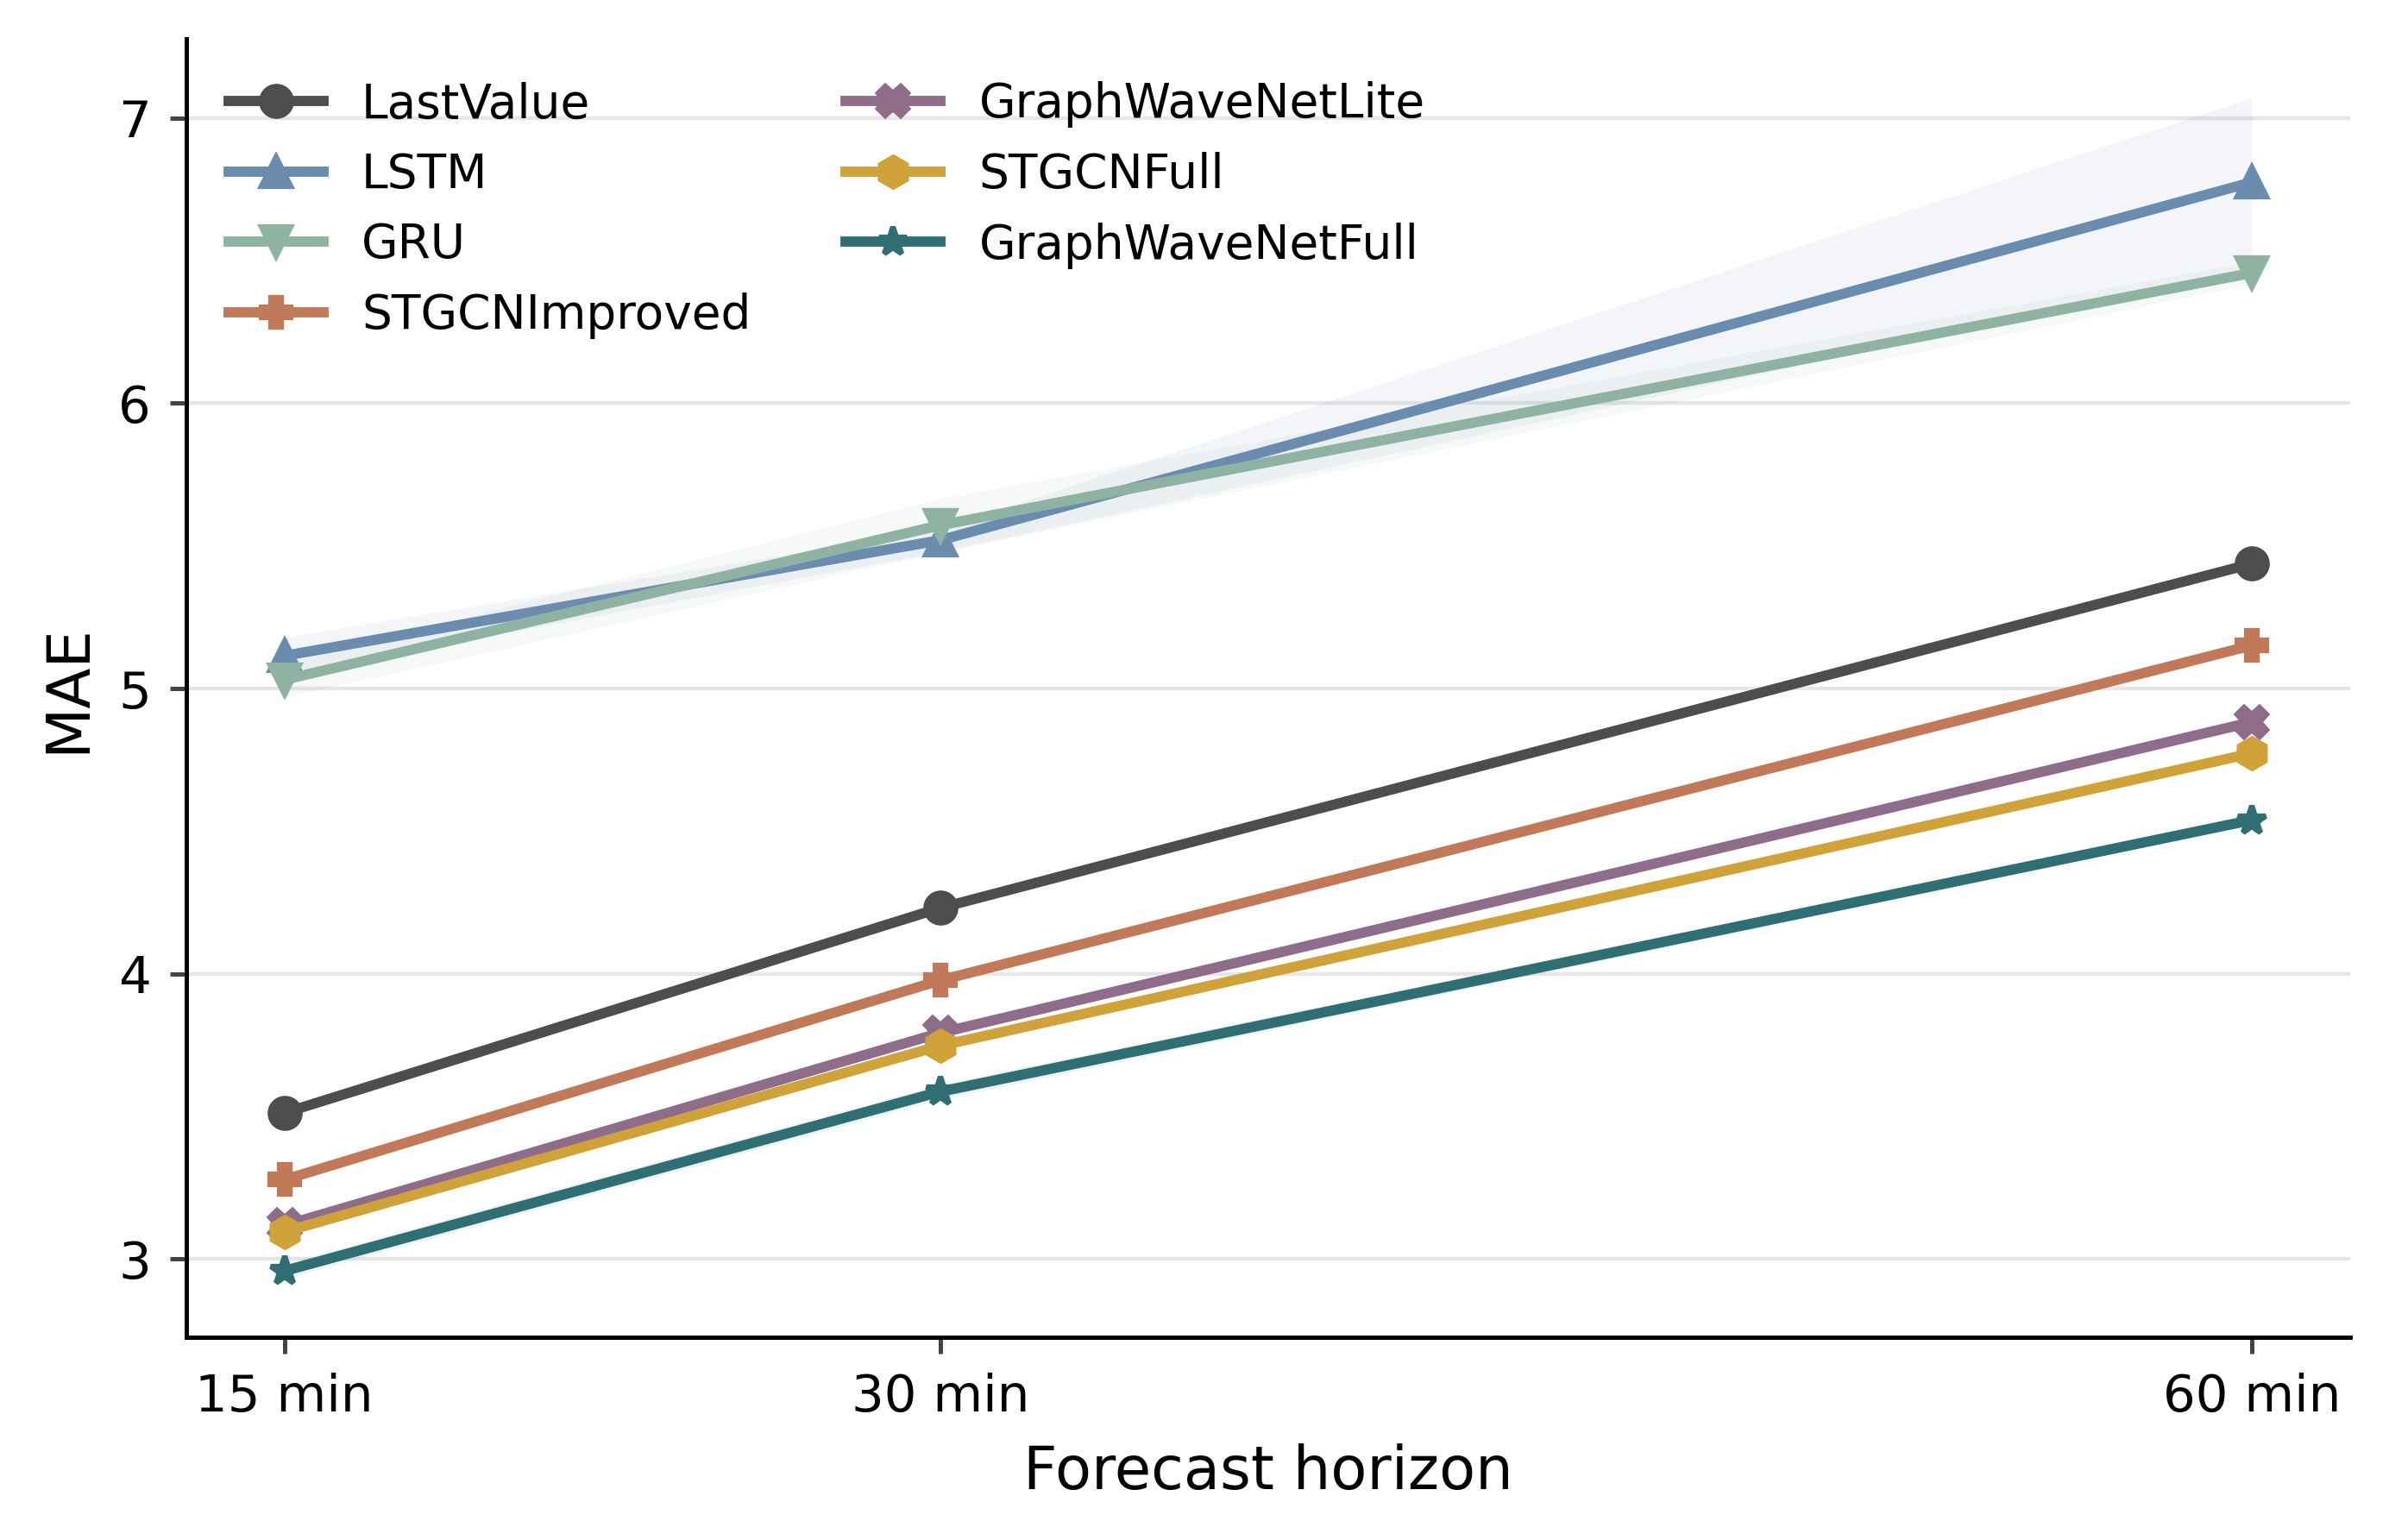
\includegraphics[width=0.82\linewidth]{../experiments/figures/METR-LA_MAE_by_Horizon.png}
  \caption{MAE across forecasting horizons.}
  \label{fig:mae_horizon}
\end{figure}

\begin{figure}[htbp]
  \centering
  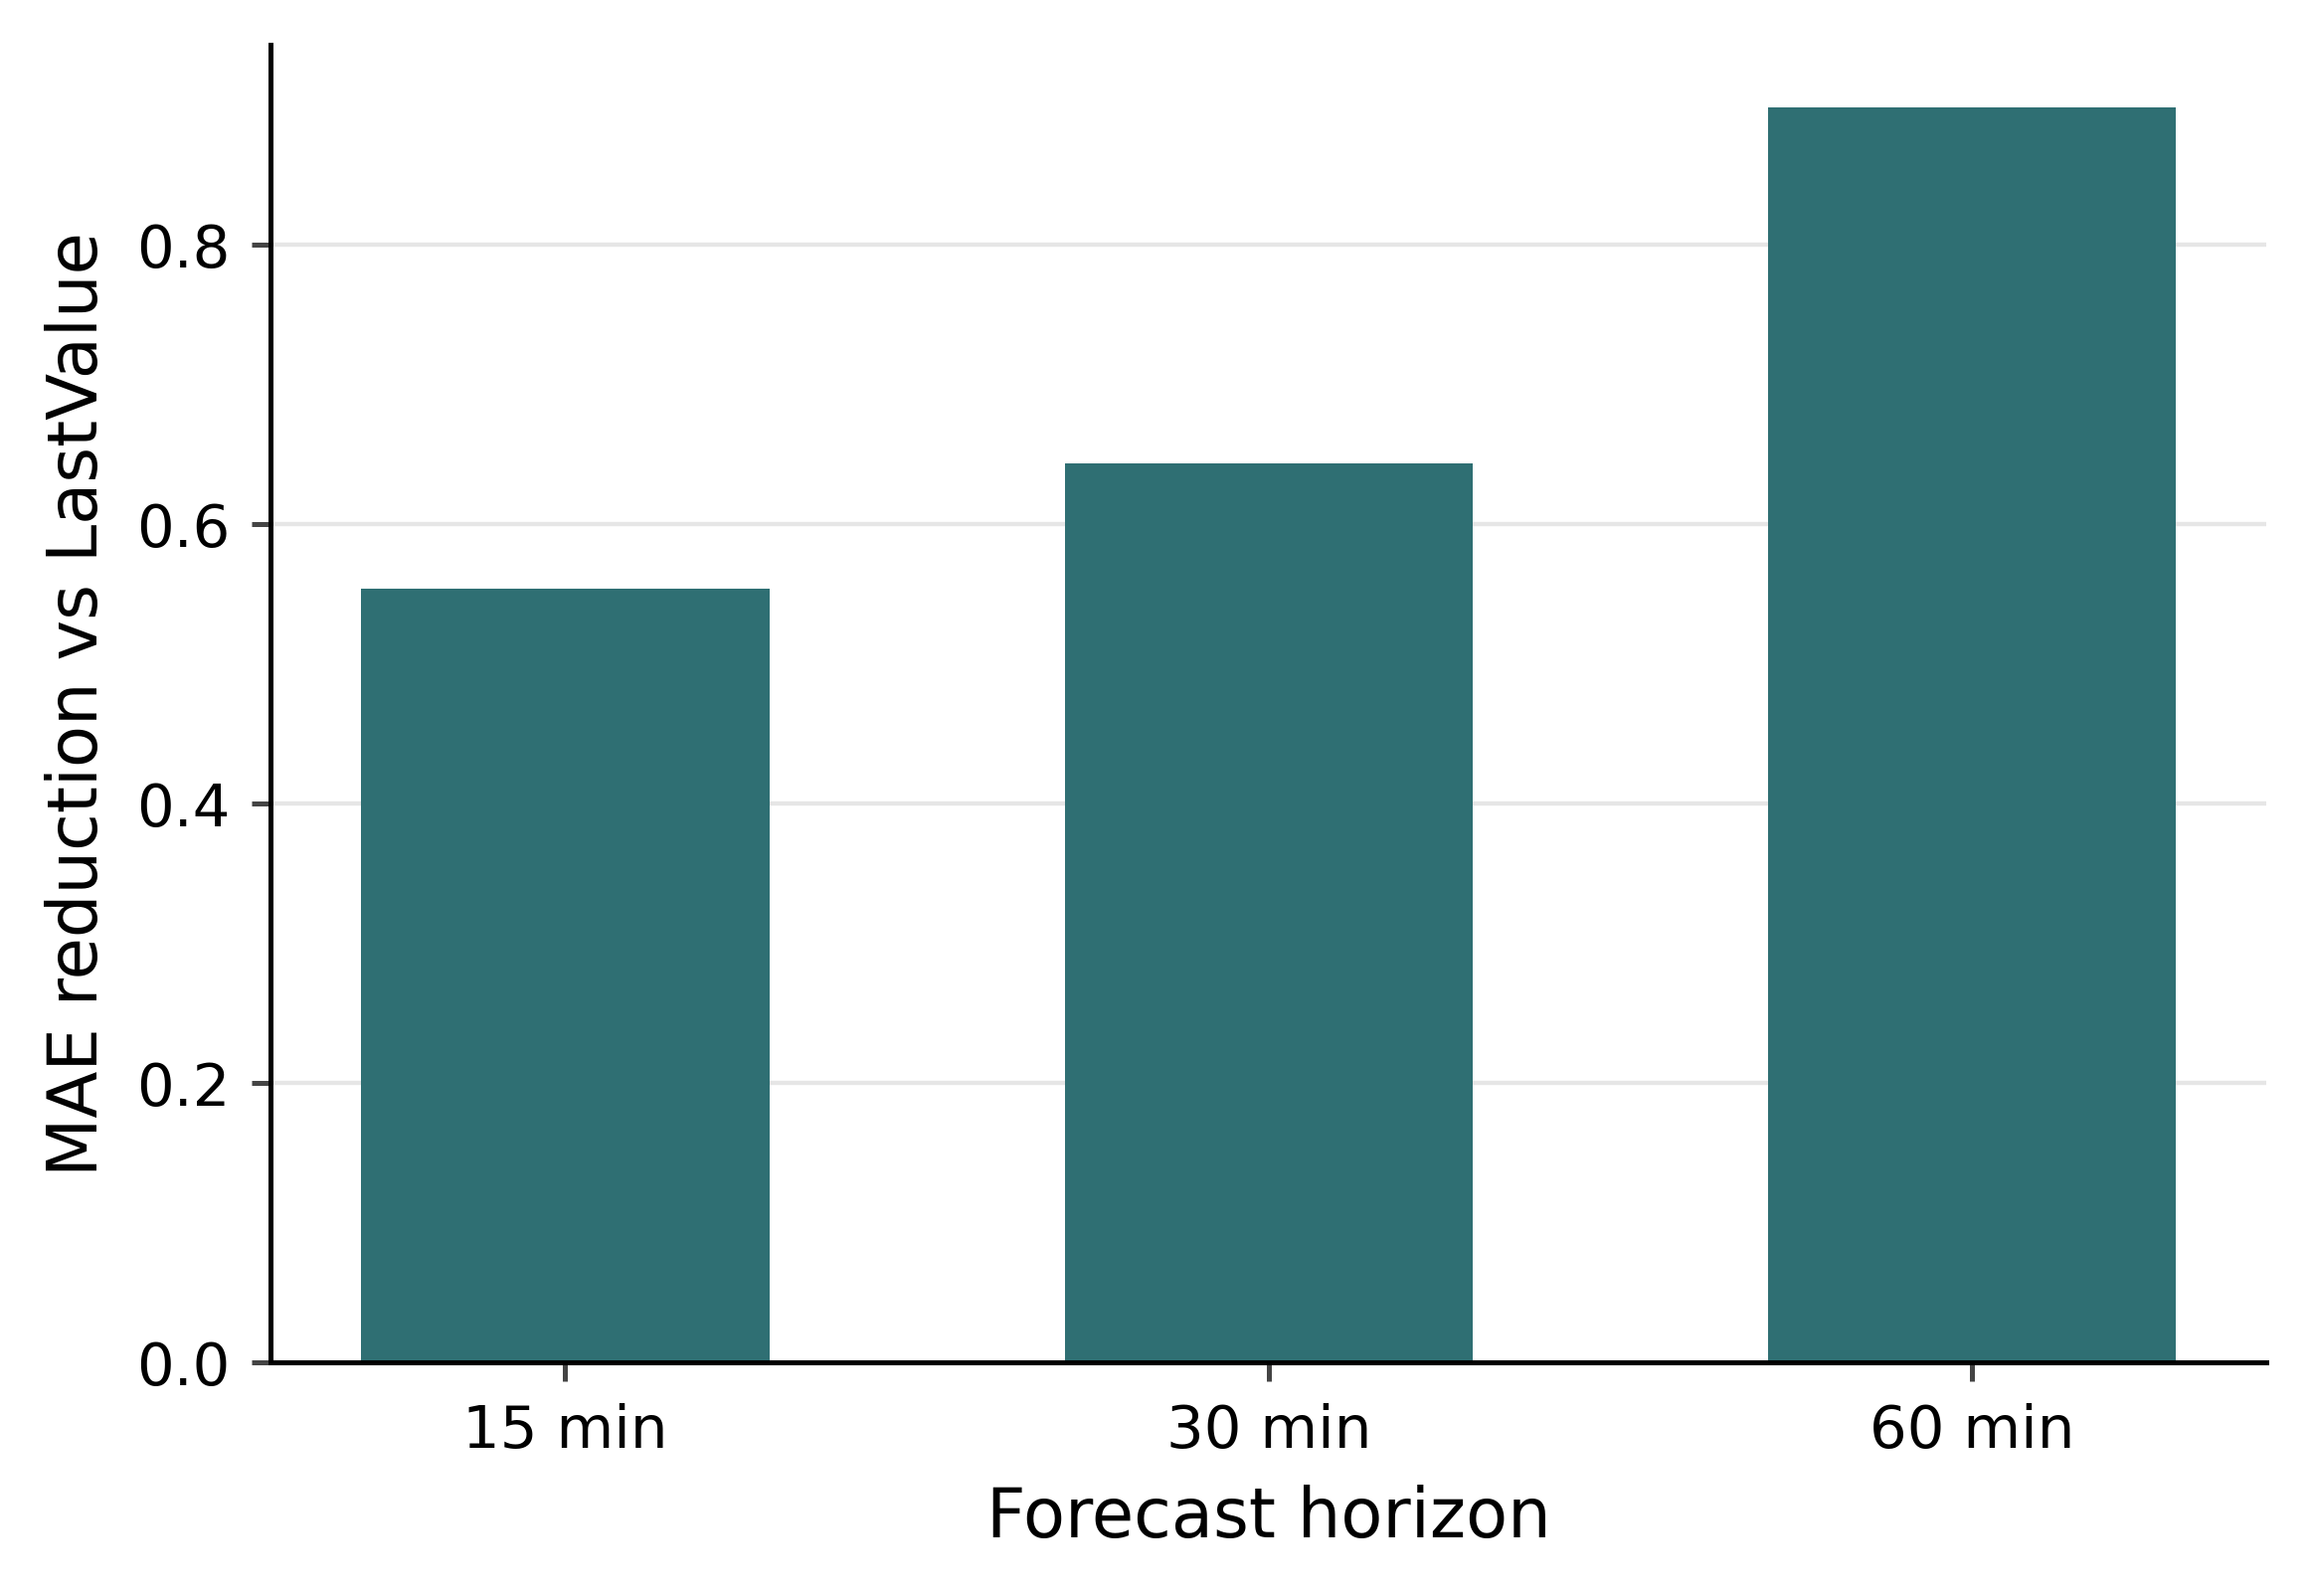
\includegraphics[width=0.82\linewidth]{../experiments/figures/GraphWaveNetFull_MAE_Reduction_vs_LastValue.png}
  \caption{MAE reduction of GraphWaveNetFull relative to LastValue.}
  \label{fig:mae_reduction}
\end{figure}

\section{Graph-Structure Ablation}
Graph-structure ablation compares identity, physical, correlation, and adaptive graph settings. Identity removes spatial coupling and approximates a no-graph condition. Physical uses the METR-LA road-topology adjacency. Correlation uses a data-driven graph estimated from the training segment only, avoiding test leakage. Adaptive graph structure is applicable to GraphWaveNet-style models with learnable node embeddings.

Table~\ref{tab:ablation} summarizes the best graph type by model and horizon according to MAE. GraphWaveNetFull performs best with adaptive/physical graph settings. STGCNFull benefits from physical topology at 15 and 30 minutes, while correlation is slightly better at 60 minutes. STGCNImproved consistently favors the physical graph. GraphWaveNetLite favors correlation in this run, suggesting that simpler graph models can sometimes benefit from data-driven similarity graphs, although this does not invalidate the usefulness of physical topology for the full models.

\begin{table}[htbp]
\centering
\caption{Best graph type by model and horizon under graph-structure ablation. Lower MAE is better.}
\label{tab:ablation}
\begin{tabular}{llrrr}
\toprule
Model & Best Graph & Horizon & MAE & masked MAPE \\
\midrule
GraphWaveNetFull & adaptive/physical & 15 min & 2.9683 & 6.6080 \\
GraphWaveNetFull & adaptive/physical & 30 min & 3.5881 & 7.8489 \\
GraphWaveNetFull & adaptive/physical & 60 min & 4.5191 & 9.6320 \\
GraphWaveNetLite & correlation & 15 min & 3.1068 & 7.2337 \\
GraphWaveNetLite & correlation & 30 min & 3.7703 & 8.7044 \\
GraphWaveNetLite & correlation & 60 min & 4.8106 & 11.0375 \\
STGCNFull & physical & 15 min & 3.0910 & 7.1828 \\
STGCNFull & physical & 30 min & 3.7561 & 8.6168 \\
STGCNFull & correlation & 60 min & 4.7425 & 10.4494 \\
STGCNImproved & physical & 15 min & 3.2766 & 7.4292 \\
STGCNImproved & physical & 30 min & 3.9764 & 8.9074 \\
STGCNImproved & physical & 60 min & 5.1441 & 11.5140 \\
\bottomrule
\end{tabular}
\end{table}

The ablation results support a nuanced conclusion: graph information is generally useful, but the best graph construction is model- and horizon-dependent. The identity graph is rarely the best setting, which suggests that spatial coupling matters. At the same time, physical adjacency is not uniformly superior to correlation or adaptive adjacency, which is plausible because road connectivity and statistical dependency are related but not identical. A physical edge may encode road proximity, while a correlation edge may capture synchronized demand or recurrent network-wide patterns.

\begin{figure}[htbp]
  \centering
  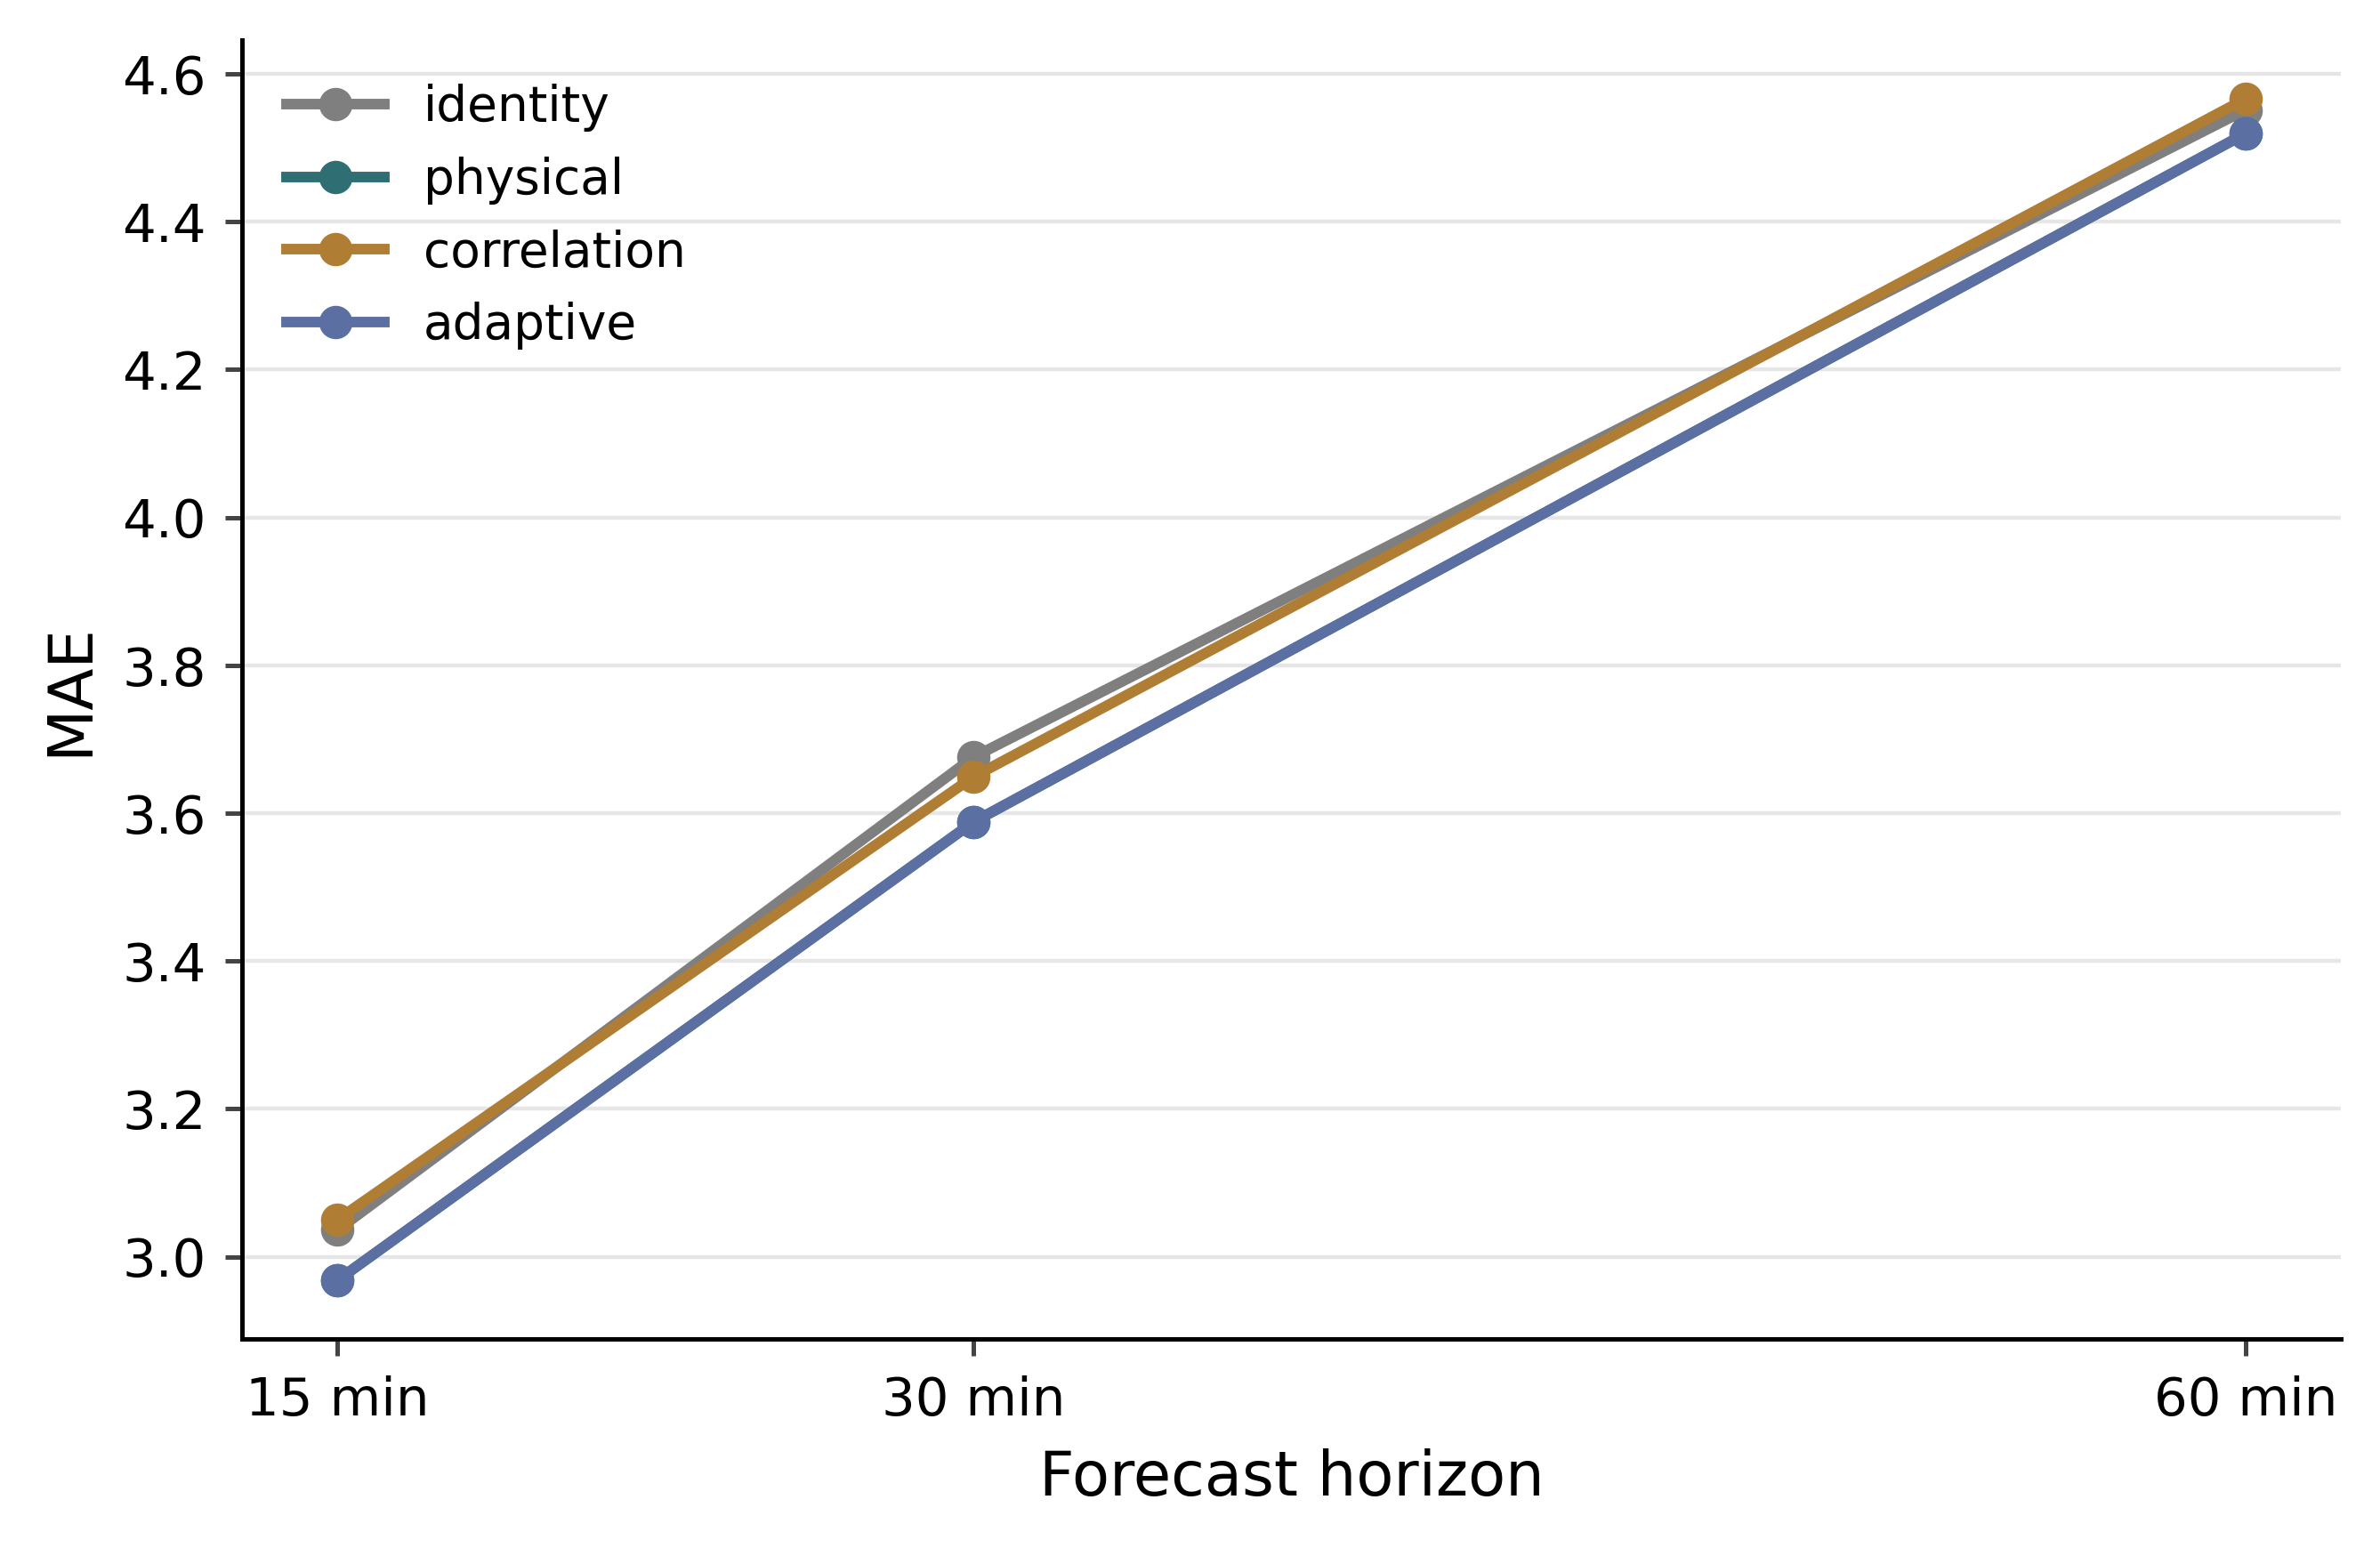
\includegraphics[width=0.82\linewidth]{../experiments/figures/GraphWaveNetFull_Graph_Ablation_MAE.png}
  \caption{GraphWaveNetFull graph-structure ablation.}
  \label{fig:graph_ablation}
\end{figure}

\section{Congestion Subset Evaluation}
Overall metrics can hide model behavior under operationally important scenarios. Therefore, the evaluation additionally defines four subsets: low speed, speed drop, high variance, and normal flow. Low-speed samples indicate congested states, speed-drop samples capture sharp degradation from recent history, high-variance samples represent unstable future windows, and normal-flow samples represent stable uncongested traffic.

When filtering to the main real-data experiments, GraphWaveNetFull gives the best MAE across the examined subsets. For example, at the 15-minute horizon it reaches MAE 4.2541 on low-speed samples and MAE 11.4046 on speed-drop samples. These subset errors are substantially larger than normal-flow errors, confirming that congestion and abrupt transitions are harder than stable traffic. This is expected: sudden speed drops are difficult for both persistence and learned models because the future departs from recent observations.

\begin{table}[htbp]
\centering
\caption{Best main-experiment congestion subset results by MAE.}
\label{tab:congestion_subset}
\begin{tabular}{llrrr}
\toprule
Subset & Best Model & Horizon & MAE & Sample Count \\
\midrule
Normal flow & GraphWaveNetFull & 30 min & 1.3958 & 3967395 \\
Low speed & GraphWaveNetFull & 15 min & 4.2541 & 901111 \\
Speed drop & GraphWaveNetFull & 15 min & 11.4046 & 275019 \\
High variance & GraphWaveNetFull & 15 min & 10.3429 & 459987 \\
\bottomrule
\end{tabular}
\end{table}

The congestion subset results should be read with caution. The subset evaluation file contains both main experiments and ablation runs; for reporting model quality, only the main experiment runs should be used. This manuscript applies that filtering. The result is still practically useful: it shows that the full graph model improves not only average prediction but also difficult traffic regimes, while also revealing that speed-drop and high-variance cases remain challenging.

\begin{figure}[htbp]
  \centering
  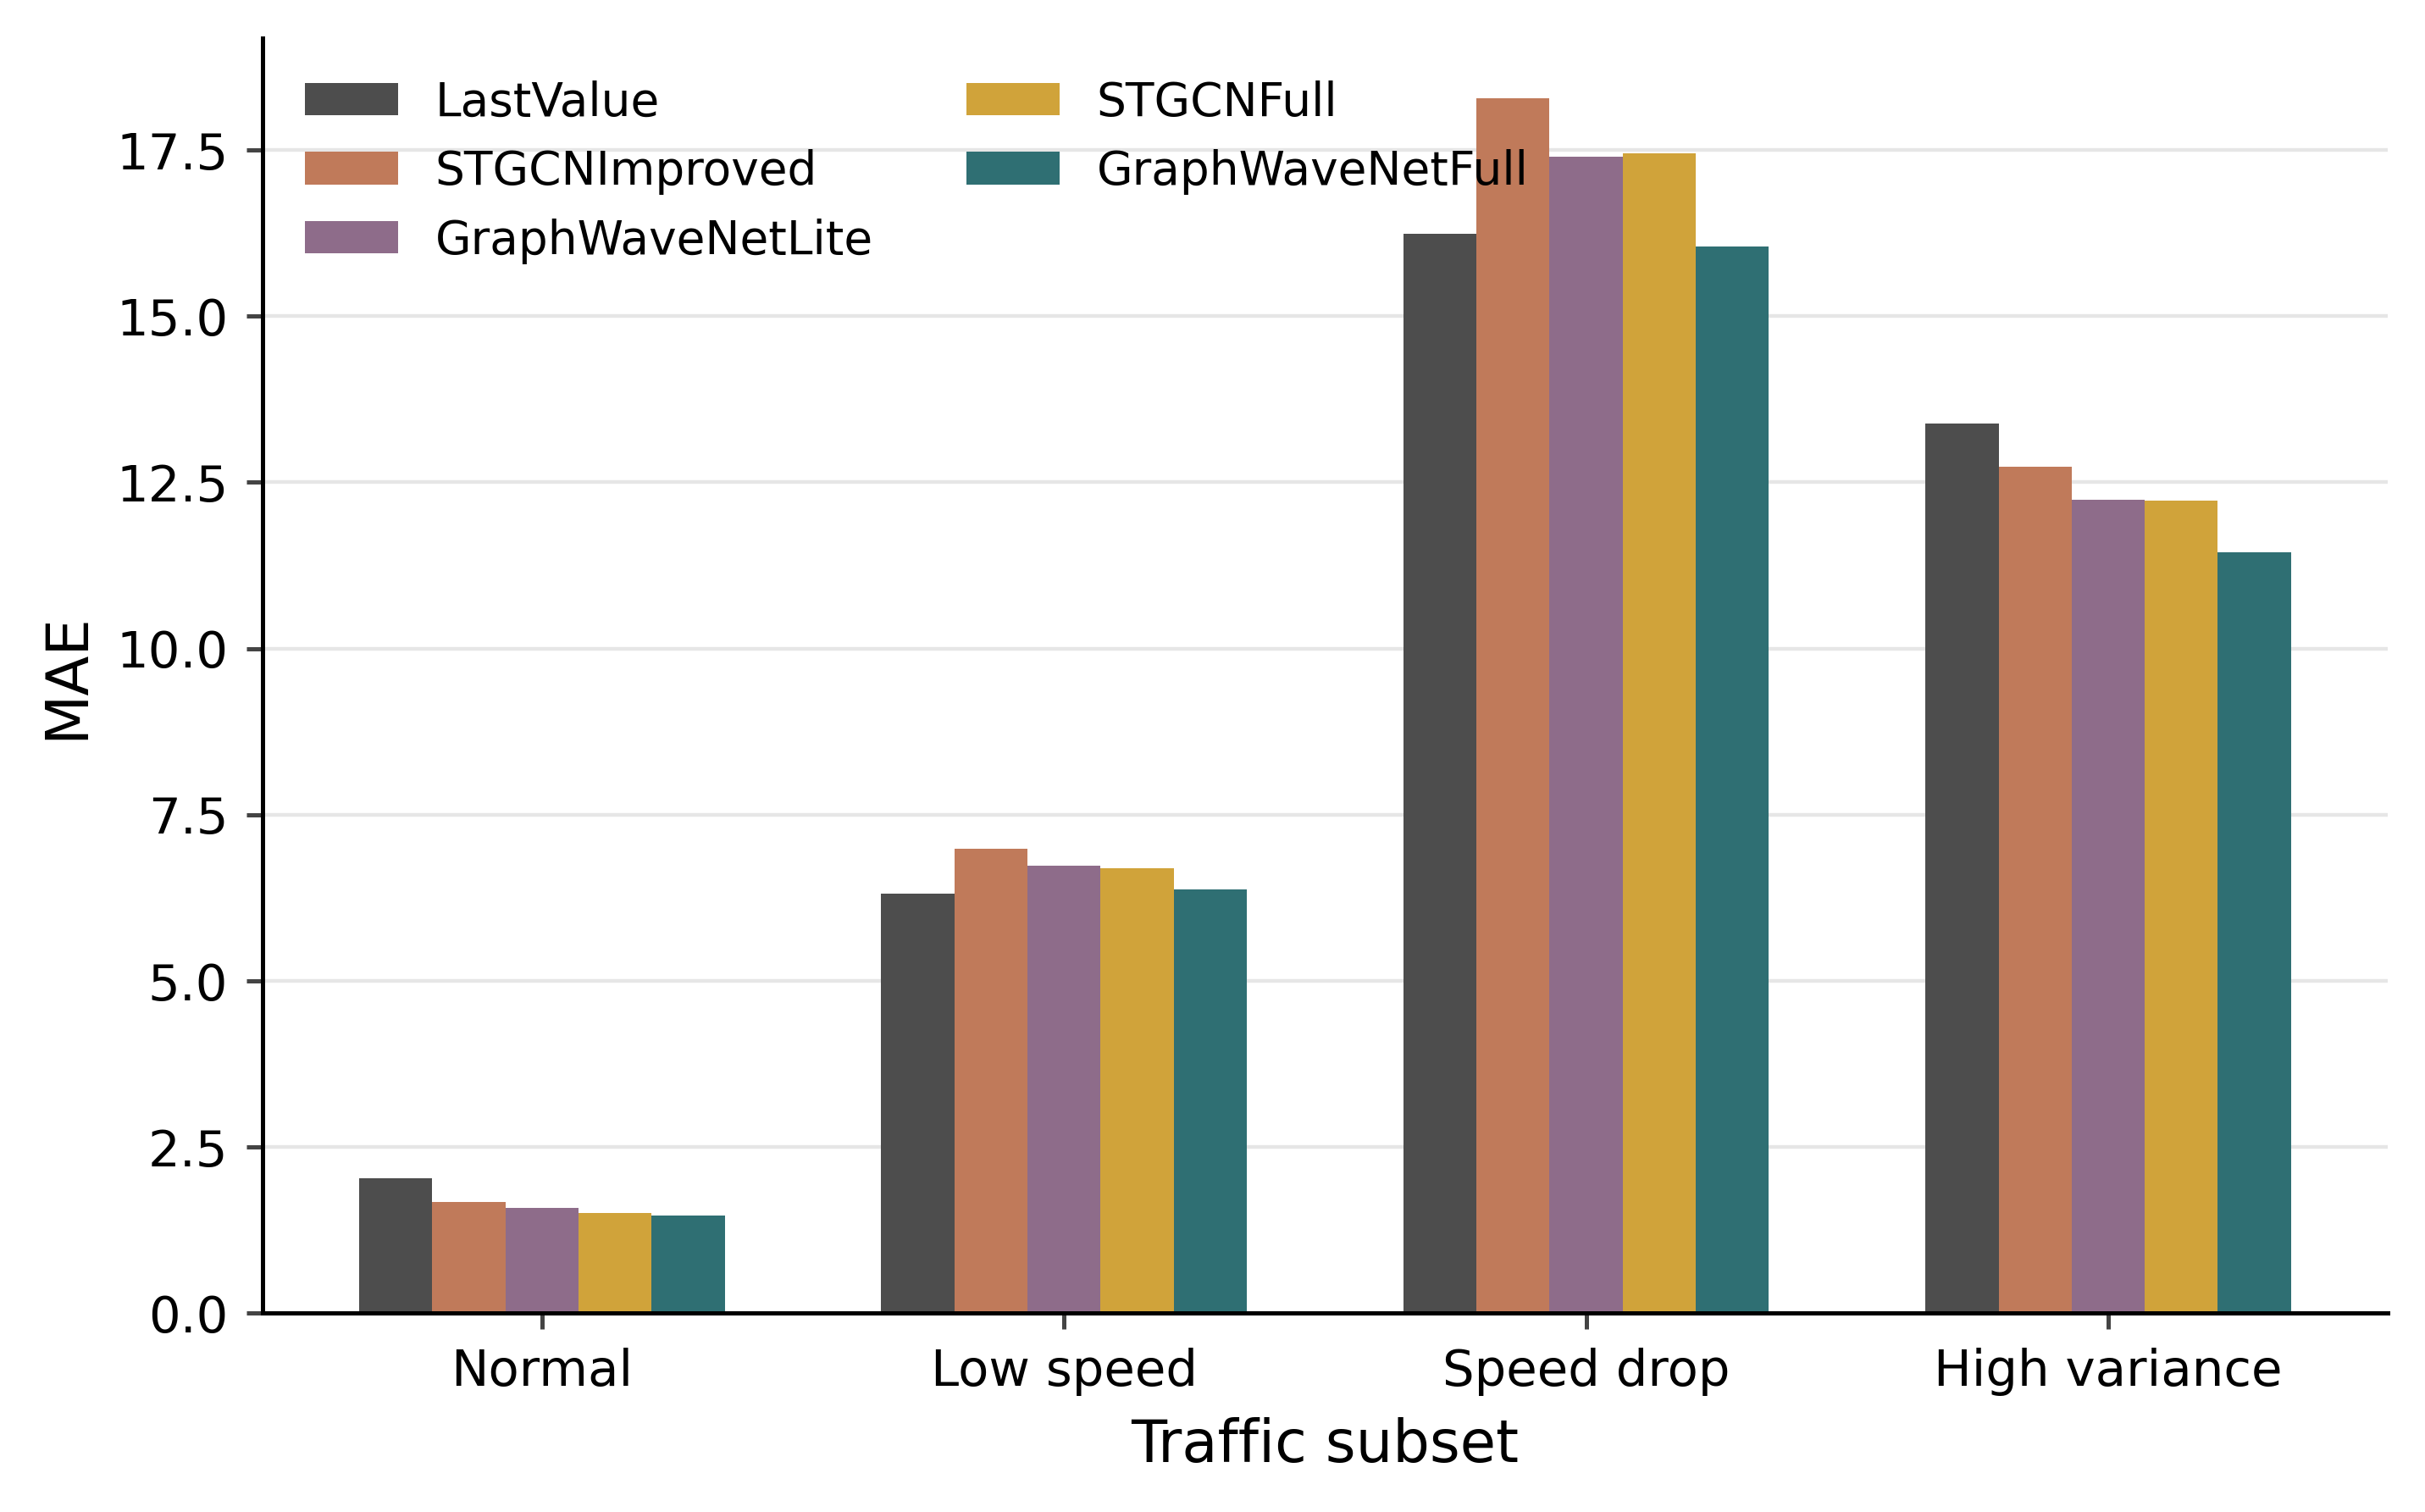
\includegraphics[width=0.82\linewidth]{../experiments/figures/Congestion_Subset_MAE_Main_Runs.png}
  \caption{MAE on congestion-oriented subsets using main experiment runs.}
  \label{fig:congestion_subset}
\end{figure}

\section{Parameter Efficiency and Model Complexity}
GraphWaveNetFull has approximately 0.73 million parameters, compared with approximately 0.19 million for STGCNFull and about 0.057 million for GraphWaveNetLite at the tested horizons. The performance improvement of GraphWaveNetFull therefore comes with higher computational and parameter cost. For portfolio and research analysis, this is acceptable because the purpose is to test whether fuller spatio-temporal structures can improve over strong baselines. For deployment-oriented scenarios, parameter count, latency, and maintenance complexity would require additional evaluation.

\begin{figure}[htbp]
  \centering
  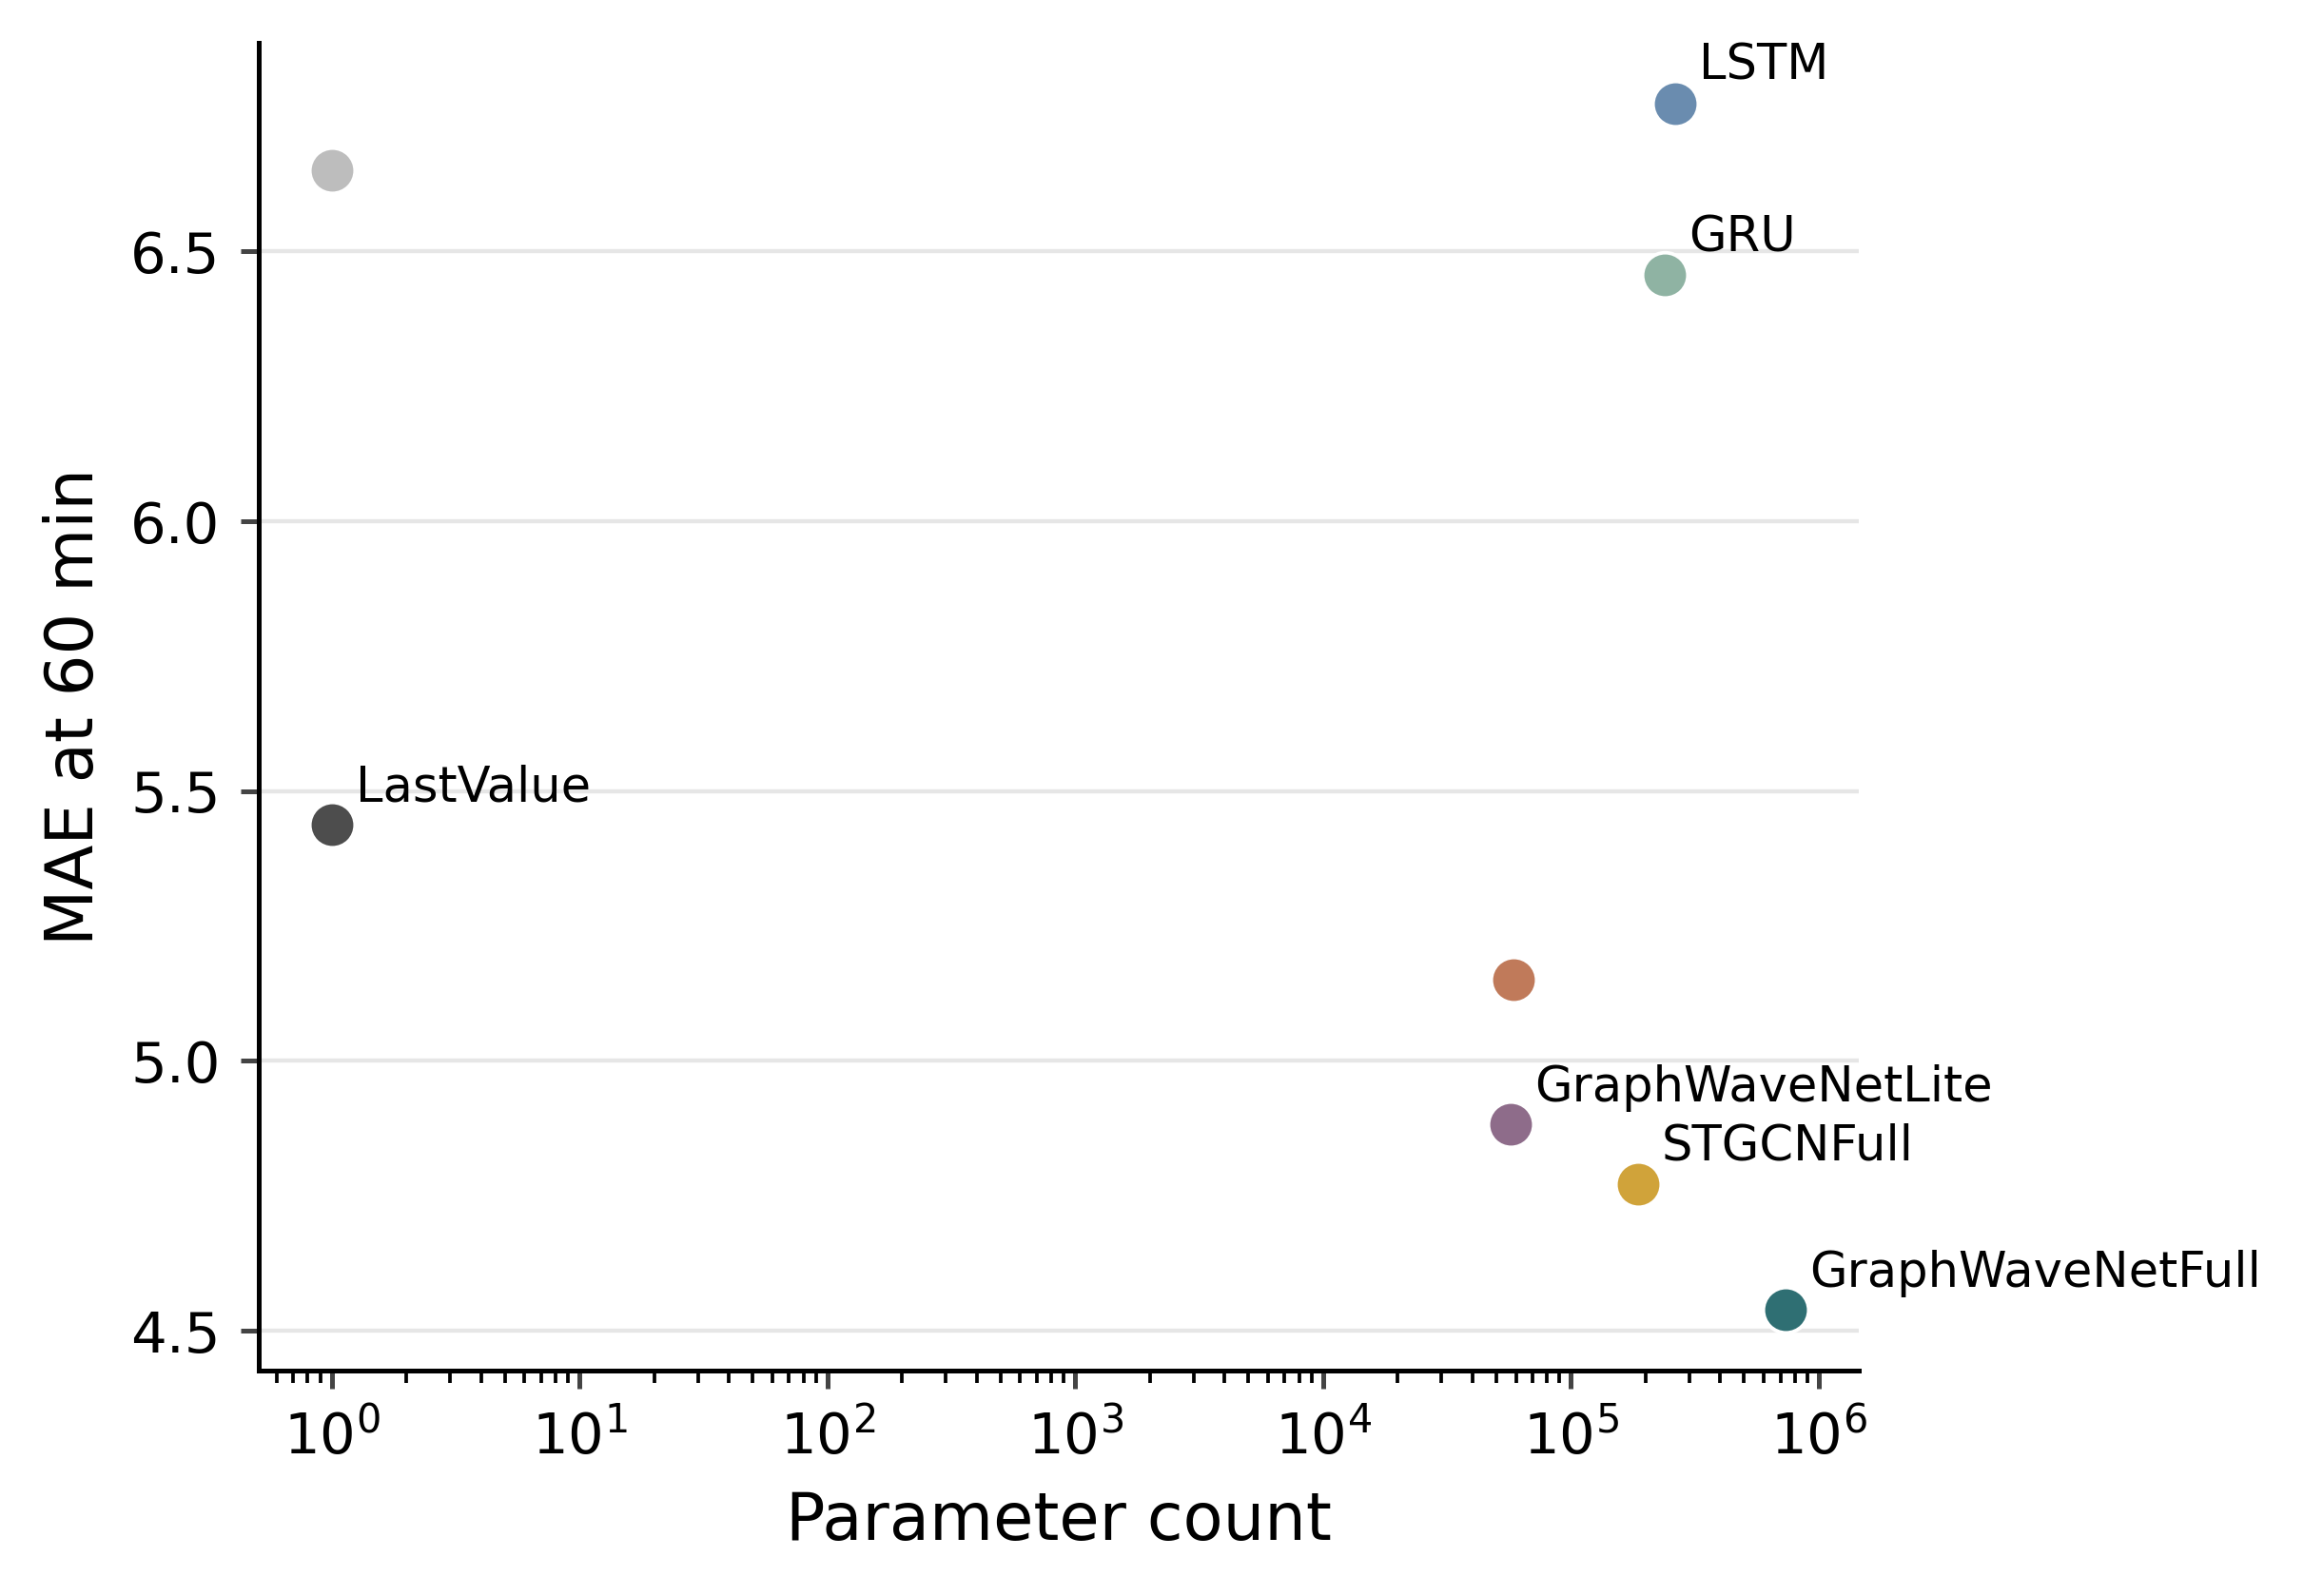
\includegraphics[width=0.78\linewidth]{../experiments/figures/Parameter_Count_vs_60min_MAE.png}
  \caption{Parameter count and 60-minute MAE tradeoff.}
  \label{fig:param_tradeoff}
\end{figure}

\section{Analysis Agent and Reporting}
The analysis agent is designed as a tool-using assistant rather than a free-form traffic-control agent. It reads stored metrics, experiment summaries, ablation tables, congestion subset results, and reports. It can answer questions such as whether full models outperform LastValue, whether graph structure helps, why raw MAPE is high, and which results are safe to describe on a resume. Each response is associated with selected tools and traceable data sources. This design prevents the agent from inventing metrics that do not exist in the output directory.

The agent also enforces a safety boundary: the system is for offline analysis and learning, not real-time traffic control. It cannot replace transportation authorities, cannot issue signal-control commands, and should not be described as a deployed operational control system.

\section{Discussion}
\subsection{Why LastValue Remains Important}
Even though GraphWaveNetFull outperforms LastValue in this experiment, LastValue remains an essential baseline. Traffic speed over a 15-minute horizon often changes slowly, so persistence is difficult to beat. A model that only improves over HistoricalAverage but not LastValue would provide weak evidence of useful short-term forecasting. The observed improvement over LastValue therefore strengthens the result, especially because it is consistent across horizons and seeds.

\subsection{Why Raw MAPE Is Not the Main Metric}
Raw MAPE can be extremely large when true speed values approach zero. This makes it sensitive to a small number of near-zero denominators. In congestion analysis, low speeds are important, but raw percentage errors should not dominate interpretation. MAE, RMSE, and masked MAPE provide more stable and interpretable evidence.

\subsection{What the Graph Ablation Shows}
The ablation study supports the hypothesis that graph structure helps, but it does not prove that physical topology is always best. Traffic dependency can arise from topology, shared demand patterns, signal coordination, and network-wide rush-hour effects. Therefore, physical, correlation, and adaptive graphs capture different aspects of traffic structure. The full conclusion should be conditional: graph modeling is beneficial in this setup, while the optimal graph support depends on model architecture and forecast horizon.

\subsection{Why Full Models Improve Over Lite Models}
The full models contain architectural mechanisms absent or simplified in the lite versions. GraphWaveNetFull uses a deeper dilated temporal stack, gated activation, skip connections, multi-support graph diffusion, and adaptive adjacency. These components likely help capture multi-scale temporal dependencies and heterogeneous node interactions. The performance gap between GraphWaveNetFull and GraphWaveNetLite is therefore plausible. However, the present implementation is not an official reproduction, and no claim is made about matching paper-reported benchmark performance.

\section{Threats to Validity}
Several limitations must be acknowledged. First, the experiments are conducted on METR-LA only; conclusions may not generalize to other cities, sensor networks, or data collection regimes. Second, the full models are paper-inspired implementations rather than faithful official reproductions with identical preprocessing, hyperparameters, and evaluation scripts. Third, no exhaustive hyperparameter search is performed, so model rankings may change under broader tuning. Fourth, congestion subset definitions are heuristic and should not be interpreted as incident detection. Fifth, the system performs offline forecasting and analysis only; it is not validated for real-time traffic management or signal control.

\section{Conclusion}
This work presents a reproducible traffic forecasting and congestion analysis project that integrates real-data processing, spatio-temporal graph forecasting, graph ablation, congestion subset evaluation, visualization, and traceable agent-based reporting. On METR-LA, GraphWaveNetFull achieves the best MAE across 15-, 30-, and 60-minute horizons and improves over the strong LastValue baseline. Graph ablation indicates that spatial structure is useful, while also showing that physical, correlation, and adaptive graphs have model-dependent advantages. Congestion subset evaluation confirms that low-speed and speed-drop regimes remain challenging but benefit from the full graph model in the main experiment setting.

The central value of the project is not a claim of state-of-the-art performance, but a disciplined experimental workflow: strong baselines, real-data node alignment, multi-seed evaluation, graph ablation, failure-aware analysis, and conservative reporting. This makes the system suitable for learning, internship portfolio demonstration, and offline traffic analytics research practice.

\appendix
\section{Reproducibility Commands}
The following commands reproduce the major experiment stages after preparing METR-LA files locally:
\begin{verbatim}
python -m traffic_agent.data.prepare_real_dataset \
  --dataset metr-la \
  --traffic-file data/raw/METR-LA/metr-la.h5 \
  --adj-file data/raw/METR-LA/adj_mx.pkl \
  --output data/processed/metr_la.npz

python -m traffic_agent.training.run_experiments \
  --config configs/metr_la_5090.yaml \
  --models last_value historical_average seasonal_naive gru lstm \
           stgcn_improved graph_wavenet_lite stgcn_full graph_wavenet_full \
  --horizons 3 6 12 \
  --seeds 42 43 44 \
  --output experiments/results/metr_la_5090_full_summary.csv

python -m traffic_agent.training.run_ablation \
  --config configs/metr_la_5090.yaml \
  --models stgcn_full graph_wavenet_full graph_wavenet_lite stgcn_improved \
  --horizons 3 6 12 \
  --seeds 42 43 44 \
  --graph-types identity physical correlation adaptive \
  --output experiments/results/metr_la_5090_ablation_summary.csv

python -m traffic_agent.analysis.congestion_eval \
  --runs-dir outputs \
  --output experiments/results/metr_la_congestion_subset_eval.csv
\end{verbatim}

\begin{thebibliography}{9}
\bibitem{li2018dcrnn}
Y. Li, R. Yu, C. Shahabi, and Y. Liu, ``Diffusion convolutional recurrent neural network: Data-driven traffic forecasting,'' in \emph{International Conference on Learning Representations}, 2018.

\bibitem{yu2018stgcn}
B. Yu, H. Yin, and Z. Zhu, ``Spatio-temporal graph convolutional networks: A deep learning framework for traffic forecasting,'' in \emph{International Joint Conference on Artificial Intelligence}, 2018.

\bibitem{wu2019graphwavenet}
Z. Wu, S. Pan, G. Long, J. Jiang, and C. Zhang, ``Graph WaveNet for deep spatial-temporal graph modeling,'' in \emph{International Joint Conference on Artificial Intelligence}, 2019.

\bibitem{kipf2017gcn}
T. N. Kipf and M. Welling, ``Semi-supervised classification with graph convolutional networks,'' in \emph{International Conference on Learning Representations}, 2017.

\bibitem{hochreiter1997lstm}
S. Hochreiter and J. Schmidhuber, ``Long short-term memory,'' \emph{Neural Computation}, vol. 9, no. 8, pp. 1735--1780, 1997.

\bibitem{cho2014gru}
K. Cho et al., ``Learning phrase representations using RNN encoder--decoder for statistical machine translation,'' in \emph{Conference on Empirical Methods in Natural Language Processing}, 2014.
\end{thebibliography}

\end{document}
